\documentclass[a4,12pt]{article}
\usepackage[parfill]{parskip}
\usepackage{placeins}
\usepackage{tabularx} % extra features for tabular environment
\usepackage{amsmath}  % improve math presentation
\usepackage{graphicx} % takes care of graphic including machinery
\usepackage[margin=1in,letterpaper]{geometry} % decreases margins
\usepackage{cite} % takes care of citations
\usepackage[final]{hyperref} % adds hyper links inside the generated pdf file
\usepackage{filecontents}
\usepackage{natbib}
\usepackage{algorithm}
\usepackage[noend]{algpseudocode}
\usepackage{algpseudocodex}
\algrenewcommand\algorithmicrequire{\textbf{Input:}}
\algrenewcommand\algorithmicensure{\textbf{Output:}}
\usepackage{blindtext}
\usepackage{amsthm}
\usepackage{amsfonts}
\usepackage{nameref,hyperref}
\usepackage{mathtools}
\usepackage{MnSymbol}
\DeclareMathOperator{\lca}{lca}
\newcommand{\Rone}{\ensuremath{\protect\overrightarrow{1}}} 
\newcommand{\rsat}{\emph{Fitch-sat}\xspace}
\newcommand{\mcEs}{\ensuremath{\mathcal{E}^{*}}}
\newcommand{\XX}[1]{\normalfont{\upshape{#1}}}
\newcommand{\btwn}{\mathop{::}}   % what is between two vertices
\newcommand{\noedge}{\mathop{\text{\textvisiblespace}}}
\newcommand{\notleftright}{\mathrel{\ooalign{$\leftrightarrow$\cr\hidewidth$/$\hidewidth}}}
% THEOREMS
\theoremstyle{plain}
\newtheorem*{theorem*}{Theorem}
\newtheorem{theorem}{Theorem}
\numberwithin{theorem}{section}
\newtheorem{lemma}[theorem]{Lemma}
\newtheorem{corollary}[theorem]{Corollary}
\newtheorem{conjecture}[theorem]{Conjecture}
\newtheorem{problem}[theorem]{Problem}
\newtheorem{remark}[theorem]{Remark}
\newtheorem{definition}{Definition}

\usepackage{listings}

%%% TO BE DELETED: %%%%%%%%%%%%%%%%%%%%%%%%%%%%%%%%%%%%%%%%%%%%%%555
\usepackage{color}
\newcommand{\TODO}[1]{\begingroup\color{red}#1\endgroup}
\newcommand{\OLD}[1]{\begingroup\tiny\color{gray}#1\endgroup}
\newcommand{\bs}[1]{\begingroup\color{blue}#1\endgroup}
\newcommand{\PFS}[1]{\begingroup\color{green}#1\endgroup}
\newcommand{\ak}[1]{\begingroup\color{orange}#1\endgroup}
\newcommand{\jr}[1]{\begingroup\color{purple}#1\endgroup}

\newcommand{\change}[1]{\begingroup\color{red}#1\endgroup}

%%% TO BE DELETED: %%%%%%%%%%%%%%%%%%%%%%%%%%%%%%%%%%%%%%%%%%%%%%555
%++++++++++++++++++++++++++++++++++++++++


\begin{document}

\title{Clustering of ITS Graphs}
\author{Thomas Gatter, Tieu Long Phan, Bruno Schmidt, Peter F. Stadler}
\date{\today}
\maketitle


\section{Introduction}

Chemical reactions, by definition, comprise the rearrangement of bonds
among the atoms of a set of reactant molecules. That is, chemical reactions
preserve the atoms involved. This fundamental property is formalized by an
atom-to-atom map (AAM). Mathematically, an AAM is simply a bijection
between corresponding atoms in the reactants and products that preserves
atom types. From a chemical point of view, the AAM encodes the
mechanism of the reaction by implying the bonds that are formed and
broken, thereby providing a condensed description of the transition from
reactants to products.

In practice, chemical reactions are typically
represented as transformations of a multiset of reactant
molecules into a corresponding multiset of product molecules. The
mechanism of a reactions, i.e., the bonds broken and newly formed, and,
equivalently, the correspondence of the atoms in reactants and products, is
not apparent from such data. In many practical applications, for instance
the analysis of isotope labeling experiments, the inference of reaction
rules, and in metabolic engineering, however, it is key to track
atoms across a reaction. To this end, structural formulas of reactants and
products, respectively, are viewed as graphs $G$ and $H$ with vertices labeled
by atom types $a$ and edges labeled by bond types $b$. The atom map of the
reaction transforming $G$ to $H$ then is a bijection $\alpha$ : $V(G) \rightarrow V(H)$ that
preserves atom types. By specifying the corresponding atoms in reactants
and product, $\alpha$ implies the bonds that are broken and formed. 
Determining the atom map of a chemical reaction given only the structural
formulas of the reactants $G$ and products $H$ is a very challenging problem.
For this lab course we provide atom maps for all reactions, and proceed under the assumption they are sufficiently correct

We encode $\alpha$ in a simple, suitable labeled graph $\Upsilon(G, H, \alpha)$,
dubbed the imaginary transition state (ITS) graph (see Fig. \ref{fig:its}).\\

\textbf{Definition:} Let $(G, H, \alpha)$ be a triple comprising two vertex and edge
labeled graphs G and H linked by an arbitrary map $\alpha : V(G) \rightarrow V(H)$.
Then the auxiliary graph $\Gamma(G, H, \alpha)$ has vertex set $V(G) \cupdot V(H)$,
 edge set $E(G) \cupdot E(H) \cupdot E(\alpha)$ where $E(\alpha) := \{x \alpha(x)|x \in V (G)\}$,
 vertex labels $(a_G(x), 1)$ for $x \in V(G)$ and $(a_H(x), 2)$ for $x \in V(H)$ and edge labels
 $b(e) = b_G(e)$ if $e \in E(G)$, $b(e) = b_H(e)$ if $e \in E(H)$, and $b(e) =$ * with *
distinct from the vertex labels in $G$ and $H$, if $e \in E(\alpha)$.\\

\textbf{Definition:} Let $\alpha$ : $V(G) \rightarrow V(H)$ be an an atom map. Then $\Upsilon(G, H, \alpha)$
is the \textbf{imaginary transition state graph} with vertex set $V(G)$, vertex labels $a_\Upsilon (x) = a_G (x)$ for all
$x \in V(G)$, and edges $xy \in E(G)$ if and only if $xy \in G$ or $\alpha(x)\alpha(y) \in E(H)$,
and tuple edge labels

$$
b(xy) := \begin{cases}
(b (xy), b_H(\alpha(x)\alpha(y))) & if xy \in E(G) and \alpha(x)\alpha(y) \in E(H) \\
(b_G(xy), \* ) & if xy \in E(G) and \alpha(x)\alpha(y) \notin E(H) \\
(\* , b_H(\alpha(x)\alpha(y)))  & if xy \notin E(G) and \alpha(x)\alpha(y) \in E(H)
\end{cases}
$$

\begin{figure}[htp]
  \centering
  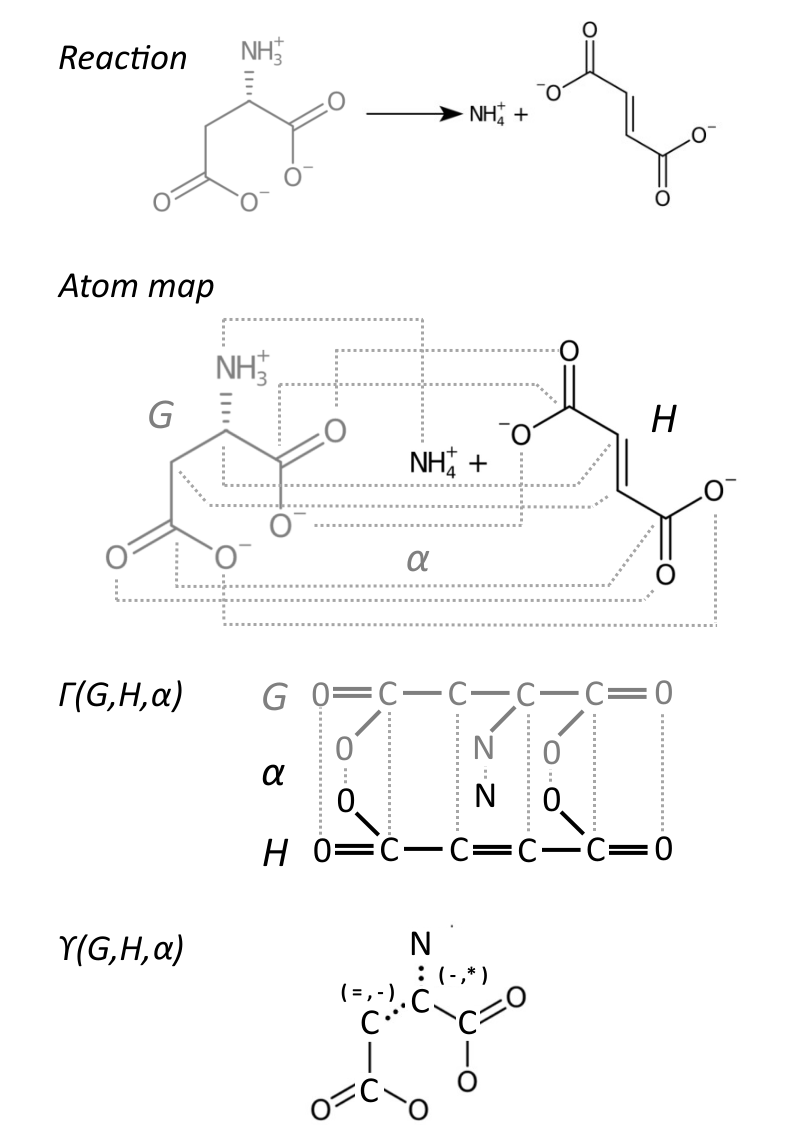
\includegraphics[width=0.6\linewidth]{images/ITS_example.png}
  \caption{\emph{From reaction to imaginary transition states:}
  Atom maps and their equivalent graphs. Top: reaction of
  the L-aspartate to fumarate and NH4+. Below,
  the chemically correct atom map $\alpha$ is shown, using dotted
  lines to connect corresponding atom. For simplicity of the
  presentation, the ammonium hydrogens are also suppresses
  in the auxiliary graphs below. $\Gamma (G, H, \alpha)$ is shown
  with vertices and edges of $G$ in gray, vertices and edges of $H$ in black,
  and the matching $E(\alpha)$ as dotted lines. In $\Upsilon(G, H, \alpha)$,
  vertices and edges with the same label in both G and H are
  drawn as full lines, while ``reaction edges'' are shown as dotted lines
  annotated by the corresponding label pairs: (=, -)
  denotes a change from a double bond to a single bond and
  (-, *) denotes the breaking of the single bond}
  \label{fig:its}
\end{figure}

As an important result, two atom maps $\alpha$ and $\beta$ are identical if an only if their corresponding ITS graphs $\Upsilon(G, H, \alpha)$ and $\Upsilon(G, H, \beta)$ are isomorphic. \\

The mechanism of a reaction is encoded by its \textbf{reaction center}, defined as the set of bonds changed between reactants and product side including respective adjacent atoms.
In an ITS graph, the reaction center is exactly the subgraph induced by the set of edges with divergent labels in the tuple.
The same chemical mechanism may appear in multiple different reactions. Although reactants and/or product compounds differ, the reaction center is constant for each mechanism. Accordingly, in order to test if two reactions use the same mechanism, and thereby belong to the same reaction class, we proceed as follows: First compute the ITS graphs of both reactions and extract the reaction centers. If the reaction centers are isomorphic, they use the same mechanism.

In the computer lab course we want to classify reactions from the USPTO database using this procedure. The goal of this course is to test methods for the effective and fast clustering of reactions. Here, clustering does not denote a grouping by distance, but rather by identity. Overall we want to solve the following task:\\
Given a set of reactions $R$, each represented by an ITS graph, compute a partition $Q_1, Q_2, \ldots, Q_N$ of unknown length $N$, such that $\bigcup\limits_i Q_i = R$ and $Q_i \cap Q_j = \emptyset$ if $i \neq j$. After the lab course, we aim to apply the implementation to a database of 10 million reactions. Clustering therefore has to be particularly fast!\\

\FloatBarrier

\section{Workpackages}\label{sec:workpackage}

\subsection{WP0}

\begin{itemize}
  \item Familiarize yourself with the definitions presented in this project description.
  \item Download the dataset from the \textit{moodle} course.
  \item For your convenience we recommend using our Python in house library SynUtils: \url{https://github.com/TieuLongPhan/SynUtils}
  \item We used the python pickle package for data preparation: \url{https://docs.python.org/3/library/pickle.html}
  \item Graph representations are based on NetworkX: \url{https://networkx.org/documentation/stable/index.html}
\end{itemize}

\subsection{WP1}

\begin{itemize}
\item Load and pre-process the provided data.
    \begin{itemize}
	\item Data is packed as Python Pickle.
	\item Reactions are given as a Python List of Dicts with following entries:
	     \begin{itemize}
	        \item \textbf{'R-id'} : ID of the USPTO database
	        \item \textbf{'class'} : USPTO database classification
	        \item \textbf{'ITS'} : NetworkX representation of the ITS Graph
		 \end{itemize}
    \item NetworkX graphs contain the following properties.
    		\begin{itemize}
    		    \item \textit{Edge:} 
    		    \item[] \textbf{'order'}: tuple of bond counts for reactant and product for this edge
    		    \item[] \textbf{'standard\_order'}: difference of bond counts between reactant and product for this edge
    		    \item  \textit{Node:} 
    		    \item[] \textbf{'charge'}: electric charge of the atom
    		    \item[] \textbf{'hcount'}: number of connected hydrogens
    		    \item[] \textbf{'aromatic'}: True if atom is in an aromatic ring
    		    \item[] \textbf{'element'}: String representation of the atom symbol
    		\end{itemize}
    \item Extract the reaction centers for each ITS. This is the induced subgraph of all edges with 'standard\_order' $\neq$ 0.
	\end{itemize}
\item Build up functions to print and/or plot reactions for manual tests later on.

\item \textbf{Hints:}\\
Loading data:
\begin{lstlisting}[language=Python]
# using only pickle
import pickle
import networkx as nx

with open('ITS_graphs.pkl.gz', 'rb') as f:
   data = pickle.load(f)
   
# using SynUtils
from synutility.SynIO.data_type import load_from_pickle

data = load_from_pickle("Data/ITS_graphs.pkl.gz")
\end{lstlisting}

Extracting reaction center and plotting using SynUtils:
\begin{lstlisting}[language=Python]
from src.rc_extract import get_rc
reaction_center = get_rc(data[0]['ITS'])

from synutility.SynVis.graph_visualizer import GraphVisualizer
import matplotlib.pyplot as plt
fig, ax = plt.subplots(2, 1, figsize = (15,10))
vis = GraphVisualizer()
vis.plot_its(data[0]['ITS'], ax[0], use_edge_color= True)
vis.plot_its(reaction_center, ax[1], use_edge_color=True)
\end{lstlisting}
\end{itemize}

\subsection{WP2}

\begin{itemize}
\item Implement a simple clustering algorithm:
\begin{itemize}
\item Input: Set of reactions $R$
\item Out: Partition $Q:=Q_1, Q_2, \ldots, Q_N$ as defined above
\item for each reaction r in R:
\begin{itemize}
\item[] let rc be the reaction center of r
\item[] for each $Q_i$ in Q:
\begin{itemize}
\item[]  if rc is isomorphic to a representative of $Q_i$, add $Q_i = Q_i \cup rc$; break;
\end{itemize}
\item[]  if rc could not be added to any set, add a new set $Q_j = \{rc\}$ to $Q$
\end{itemize}
\end{itemize}
\item \textbf{Hints:}
\begin{itemize}
\item make sure only one isomorphism check is executed per rc and $Q_i$, as entries within $Q_i$ have identical reaction centers by definition
\item use the NetworkX function \textit{is\_isomorphic} with node labels 'charge' and 'element' and edge label 'order'.
\end{itemize}
\end{itemize}

\subsection{WP3}

We now want to apply pre-filters to roughly group reactions before applying WP2 on subgroups.
\begin{itemize}
\item From the lecture we know that graph invariants do not change between isormorphic graphs, granting them their name.
\item We therefore can use them to group our reactions:
\begin{itemize}
\item If the invariant is identical, reactions centers may be isomorphic, so they are added to the same cluster.
\item If the invariant is different, reactions centers cannot be isomorphic, so they must appear in different clusters.
\end{itemize}
\item Modify WP2 such that graphs are clustered not by isomorphism, but by the invariant.
\item Apply isomorphism clustering to further subdivide each invariant cluster to the final isomorphism cluster set $Q$.
\item Test various graph invariants of your liking, including at least vertex and edge counts, vertex degrees, algebraic connectivity and rank (look here for inspiration \url{https://en.wikipedia.org/wiki/Category:Graph_invariants}).
\end{itemize}

\subsection{WP4}

We want to implement (hierarchical) clustering by modifying the Weisfeiler-Lehmann Isomorphism Test. 

Version A:
\begin{itemize}
\item Use the NetworkX function \textit{weisfeiler\_lehman\_graph\_hash} as an invariant and apply WP3
\item Test different step counts by modifying the 'iterations' options.
\item Include 'edge\_attr' and 'node\_attr'. This will require an aggregated node attribute containing both 'charge' and 'element' in one string.
\end{itemize}

Version B:
\begin{itemize}
\item Implement the Weisfeiler Lehmann Isomorphism Test yourself as it was described in the lecture.
\item Make sure to use a shared hash table for concurrently tested graphs.
\item No proceed as follows:
   \begin{itemize}
   \item Compute the first Weisfeiler Lehmann  iteration for all reactions using a shared hash table. 
   \item Apply WP3 clustering using the histogram of each graph as the invariant.
   \item Now for every resulting Cluster $Q_i$ independently:
       \begin{itemize}
        \item Compute the second iteration for every member of $Q_i$.
        \item You may use an independent copy of the hash table from the last step only shared for $Q_i$.
        \item Apply WP3 on the resulting histograms to further subdivide $Q_i$ into smaller clusters  
       \end{itemize}
   \item Apply this procedure recursively to subdivide clusters until a threshold cluster size or a maximum number of iterations is reached. 
   \item Apply isomorphism clustering on each resulting cluster independently to create the final isomorphic cluster set.
   \end{itemize}
\end{itemize}


\subsection{WP5}

\begin{itemize}
\item Document and benchmark all of the previous work packages.
\item What are the clustering times?
\item What graph invariants lead to a good partition and which don't?
\end{itemize}


%\bibliographystyle{plainnat}
%\bibliography{lib.bib}

\end{document}
